\begin{figure}[ht!]
\small
\begin{center}
\setlength{\tabcolsep}{1pt}
\begin{tabular}{cccc}
\hspace{3mm} Task OSSE & 
\hspace{3mm} Task OSSE & 
\hspace{2mm} Task OSSE & 
Task OSE \\
\hspace{3mm}  Nadir & 
\hspace{3mm} Nadir + SWOT & 
\hspace{2mm} Nadir + SST & 
Nadir \\
%\vspace{-2mm}
%%%%% SSH %%%%%%%%
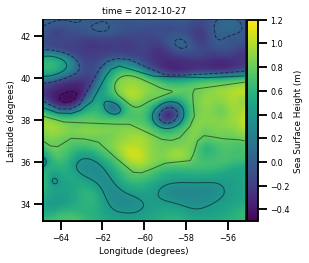
\includegraphics[trim={0 13mm 22mm 0},clip, width=3.60cm,height=3.2cm]{00_Oceanbench/content/figures/fourdvarnet_figs/osse_gf_nadir_ssh.png} &
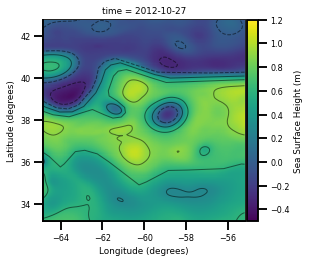
\includegraphics[trim={13mm 13mm 22mm 0},clip, width=3.2cm,height=3.2cm]{00_Oceanbench/content/figures/fourdvarnet_figs/osse_gf_nadirswot_ssh.png} &
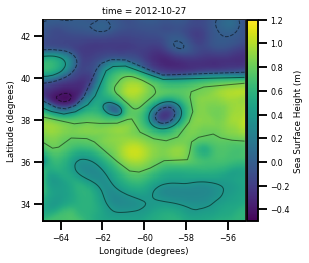
\includegraphics[trim={13mm 13mm 22mm 0},clip, width=3.2cm,height=3.2cm]{00_Oceanbench/content/figures/fourdvarnet_figs/osse_gf_nadir_sst_ssh.png} &
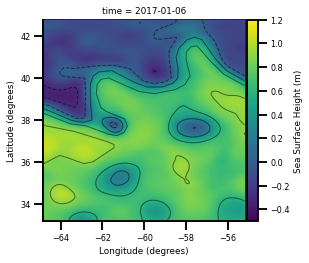
\includegraphics[trim={13mm 13mm 0 0},clip,width=4.0cm,height=3.2cm]{00_Oceanbench/content/figures/fourdvarnet_figs/ose_gf_ssh.png} \\
%\vspace{3mm}
%%%%% KINETIC ENERGY %%%%%%%%
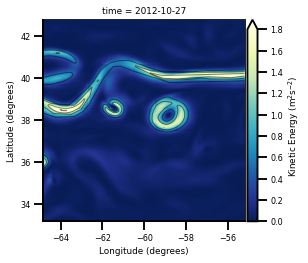
\includegraphics[trim={0 13mm 22mm 5mm}, clip, width=3.60cm,height=3cm]{00_Oceanbench/content/figures/fourdvarnet_figs/osse_gf_nadir_ke.png} &
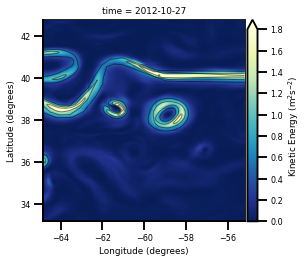
\includegraphics[trim={13mm 13mm 22mm 5mm},clip, width=3.2cm,height=3cm]{00_Oceanbench/content/figures/fourdvarnet_figs/osse_gf_nadirswot_ke.png} &
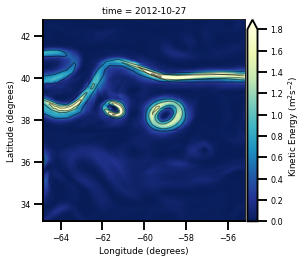
\includegraphics[trim={13mm 13mm 22mm 5mm},clip, width=3.2cm,height=3cm]{00_Oceanbench/content/figures/fourdvarnet_figs/osse_gf_nadir_sst_ke.png} &
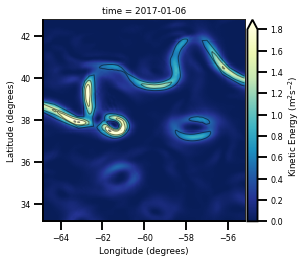
\includegraphics[trim={13mm 13mm 0 5mm},clip,width=4cm,height=3cm]{00_Oceanbench/content/figures/fourdvarnet_figs/ose_gf_ke.png} \\
%%%%% RELATIVE VORTICITY %%%%%%%%
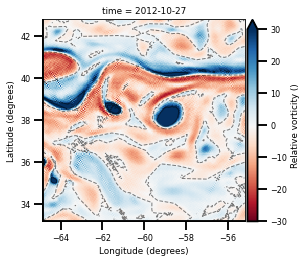
\includegraphics[trim={0 13mm 21.2mm 5mm},clip, width=3.60cm,height=3cm]{00_Oceanbench/content/figures/fourdvarnet_figs/osse_gf_nadir_vort_r.png} &
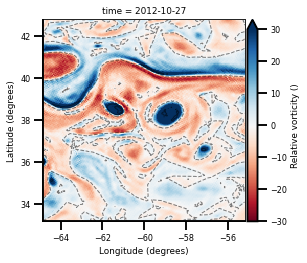
\includegraphics[trim={13mm 13mm 21.2mm 5mm},clip, width=3.2cm,height=3cm]{00_Oceanbench/content/figures/fourdvarnet_figs/osse_gf_nadirswot_vort_r.png} &
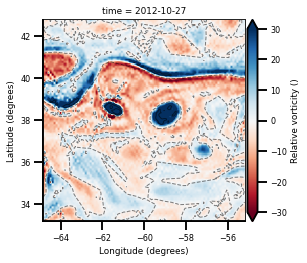
\includegraphics[trim={13mm 13mm 21.2mm 5mm},clip, width=3.2cm,height=3cm]{00_Oceanbench/content/figures/fourdvarnet_figs/osse_gf_nadir_sst_vort_r.png} &
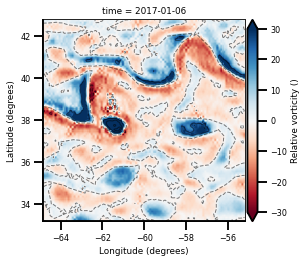
\includegraphics[trim={13mm 13mm 0 5mm},clip,width=4.0cm,height=3cm]{00_Oceanbench/content/figures/fourdvarnet_figs/ose_gf_vort_r.png} \\
%%%%% STRAIN %%%%%%%%
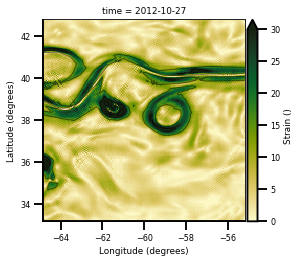
\includegraphics[trim={0 0 19mm 5mm},clip, width=3.60cm,height=3.4cm]{00_Oceanbench/content/figures/fourdvarnet_figs/osse_gf_nadir_strain.png} &
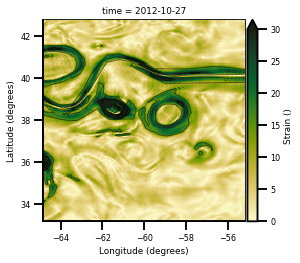
\includegraphics[trim={13mm 0 19mm 5mm},clip, width=3.2cm,height=3.4cm]{00_Oceanbench/content/figures/fourdvarnet_figs/osse_gf_nadirswot_strain.png} &
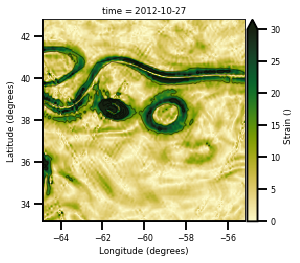
\includegraphics[trim={13mm 0 19mm 5mm},clip, width=3.2cm,height=3.4cm]{00_Oceanbench/content/figures/fourdvarnet_figs/osse_gf_nadir_sst_strain.png} &
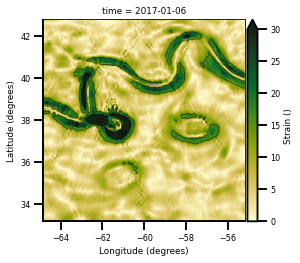
\includegraphics[trim={13mm 0 0 5mm},clip,width=4.0cm,height=3.4cm]{00_Oceanbench/content/figures/fourdvarnet_figs/ose_gf_strain.png} \\
% \vspace{-2mm}
(a) & (b) & (c) & (d)
\end{tabular}
\vspace{-3mm}
% \caption{Row I - Isotrophic PSD. Row 2 - Isotrophic PSD Score}
\caption{
Reconstructed quantities by the 4dVarNet method for each of the four tasks.
Each row showcases the following physical variables found in appendix~\ref{sec:physical_variables}: (a) Sea Surface Height, (b) Kinetic Energy, (c) Relative Vorticity, and (d) Strain. 
Each column showcase the reconstructed from the tasks (a) OSSE using only Nadir tracks: (b) OSSE using Nadir tracks and SWOT swath, (c) Multimodal using Nadir tracks and sea surface temperature, and (d) Reconstruction using real nadir altimetry tracks.}
\vspace{-5mm}
\label{fig:oceanbench_maps_4dvarnet}
\end{center}
\end{figure}